\documentclass{article}%
\usepackage[T1]{fontenc}%
\usepackage[utf8]{inputenc}%
\usepackage{lmodern}%
\usepackage{textcomp}%
\usepackage{lastpage}%
\usepackage{geometry}%
\geometry{left=2.5cm,top=1.5cm}%
\usepackage[dvipsnames]{xcolor}%
\usepackage{array}%
\usepackage{colortbl}%
\usepackage{graphicx}%
\usepackage{caption}%
\usepackage{ragged2e}%
%
%
%
\begin{document}%
\normalsize%
\section{Análisis Sísmico}%
\label{sec:AnlsisSsmico}%
\subsection{Factor de Zona}%
\label{subsec:FactordeZona}%
Esto mostrará una lista de los commits en el repositorio, comenzando con el commit más reciente.\newline%
Cada commit estará identificado por una cadena de caracteres larga y hexadecimal que aparece en la\newline%
línea que comien\newline%
%


\begin{table}[ht!]%
\begin{minipage}{0.55\textwidth}%
\caption{Factor de zona}%
\begin{tabular}{|>{\centering\arraybackslash}m{3.75cm}|>{\centering\arraybackslash}m{3.75cm}|}%
\hline%
\multicolumn{2}{|c|}{\textbf{FACTOR DE ZONA SEGÚN E{-}030}}\\%
\hline%
\textbf{ZONA}&\textbf{Z}\\%
\hline%
Zona&Z\\%
\hline%
\end{tabular}%
\end{minipage}%
\begin{minipage}{0.35\textwidth}%
\begin{center}%
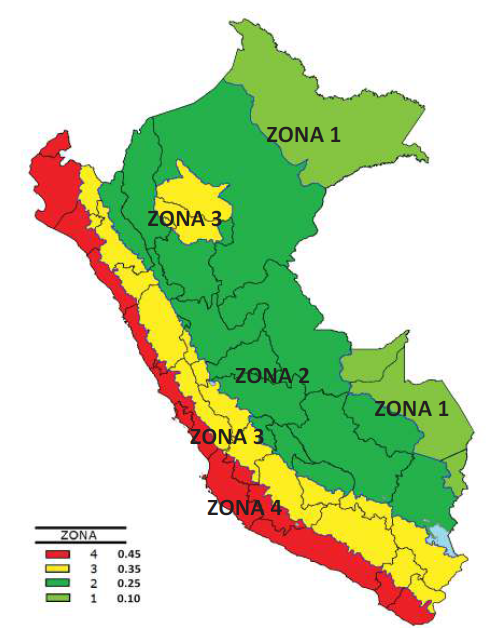
\includegraphics[width=4cm]{mapa_zona}%
\end{center}%
\end{minipage}%
\caption*{Fuente: E-30 (2018)}%
\end{table}

%
Esto mostrará una lista de los commits en el repositorio, comenzando con el commit más reciente. Cada commit estará identificado por una cadena de caracteres larga y hexadecimal que aparece en la línea que comienz

%
\end{document}